\section{Desugaring}
\label{sec:desugar}

\jeremy{don't forget we changes to CBV in the target, reflect the change in
  trait desuagr}

\name is built upon a thin-layer of sugar on top of \bname~\cite{}.
\bname is polymorphic language with subtyping, and it was developed as
an alternative to languages such as System $F_{<:}$ to serve as a core
languages for OO languages. The choice of \bname is due to its
support for disjoint intersection types and disjoint polymorhism (used
to model subtyping and conflict detection), and the so-called merged
operator (which is used to model dynamic trait inheritance).  The theoretical
aspects of \bname (including the formalization of the static and
dynamic semantics, and the proofs of type-safety and coherence) were
already studied in previous work. So they are not a contribution of
this paper and are not necessary to understand the desugaring process.

The novelty in this section is to explain how to build a high-level OO asbtractions
on top of the the core constructs of \bname. In particular we focus on
how the trait system presented in this paper is built. The key idea behind trait translation is
inspired by the functional mixin semantics using open recursion, which is
proposed by~\citet{cook1989denotational} in an untyped setting. However, our
translation is done in the context of a statically-typed programming language,
which is exactly why conflicts can be \textit{statically} detected in traits.

\subsection{A Brief Introduction to \bname}
The syntax of our core language \bname is shown in Figure~\ref{fig:synax-fi}. It
is mostly based on the calculus proposed by~\citet{alpuimdisjoint}, with several
extensions (e.g., term and type declarations, more primitive types,
etc\footnote{We have very limited support for higher-kinded types, for which we
  haven't worked out the meta-theory yet.}.)
\bruno{I think we can omit most of the primitive types and operations
  from the formal syntax. You should present the syntactic sugar for
  (multi-field) records and record types in the figure.} 
\bruno{Briefly explain the key novel contructs: merge, big lambda }
\bruno{Explain that declarations/programs are new, but we don't think
  this will cause any programs to the meta-theory.}

\begin{figure}[t]
\centering
% \begin{small}
\begin{tabular}{lrcl}
  Types  & $[[A]], [[B]]$ & ::= & $[[top]] \mid [[Int]] \mid [[Bool]] \mid [[String]] \mid [[A -> B]] \mid [[A & B]] \mid  [[{ l : A }]]  $ \\
         && $\mid$ & $[[a]] \mid [[forall ( a ** A ) . B]] \mid [[ A [ B1 ... Bn ] ]]$ \\
  Expressions & $[[E]]$ & ::= & $[[top]] \mid [[N]] \mid [[S]] \mid [[E1 + E2]] \mid [[E1 - E2]] \mid [[E1 * E2]] \mid [[E1 / E2]] \mid [[E1 ,, E2]] $ \\
         && $\mid$ & $[[BL]] \mid [[E1 == E2]] \mid [[E1 /= E2]] \mid [[E1 < E2]] \mid [[E1 > E2]] \mid [[if E1 then E2 else E3]] $ \\
         && $\mid$ & $[[x]] \mid [[\ x . E]] \mid [[E1 E2]] \mid [[blam ( a ** A ) . E]] \mid [[E A]]$ \\
         && $\mid$ & $[[{ l = E }]] \mid [[E . l]] \mid [[E -- l]] \mid [[let x : A = E1 in E2]]$ \\
  Programs & $[[pgm]]$ & ::= & $[[decl1 .. decln E]]$ \\
  Declarations & $[[decl]]$ & ::= & $[[ def f ( x1 : A1 ) .. ( xn : An ) : B = E ]] \mid [[ type T [ a1 .. an ] = A ]]$
\end{tabular}
% \end{small}
\caption{Syntax of \bname }
\label{fig:synax-fi}
\end{figure}

\subsection{Trait Declarations}

\bruno{You should put all desugarings in a single Figure.}

Essentially traits are translated into term declarations, with methods becoming
record fields. The self-reference is adjusted to be the last parameter of the
declaration. For example,
\begin{lstlisting}
  trait point(x : Int, y: Int) { self : Point =>
    def x() = x
    def y() = self.x()
  }
\end{lstlisting}
becomes
\begin{lstlisting}
  def point (x : Int) (y : Int) (self : Point) =
  { x = \_ -> x
  , y = \_ -> self.x()
  }
\end{lstlisting}
Now it is clear that \lstinline{self} is not a special keyword: it can
have any name.

Figure~\ref{fig:trans-trait} presents the translation of trait
declarations.\bruno{You should expand this a little bit. }


\begin{figure}[t]
  \centering
  \begin{tabular}{l}

\begin{lstlisting}[mathescape=true]
trait m ($x_1 : A_1$, .., $x_n : A_n$) inherits $a_1$ & .. & $a_m$ { s : $A_0$ =>
  def $m_1$(..) = $e_1$
  ..
  def $m_s$(..) = $e_s$
}
\end{lstlisting} \\

    $\rightsquigarrow$ \\

\begin{lstlisting}[mathescape=true]
def m $(x_1 : A_1)$ .. $(x_n : A_n)$ $(s : A_0)$ = $a_1$(s) ,, .. ,, $a_m$(s) ,, {
  $m_1$ = \(..) -> $e_1$
, ..
, $m_s$ = \(..) -> $e_s$
}
\end{lstlisting}
  \end{tabular}
\caption{Translating trait declaration}
\label{fig:trans-trait}

\end{figure}

\begin{figure}[t]
  \centering
  \begin{tabular}{l|l}

\begin{lstlisting}[mathescape=true]
new[$A_1$ & ... & $A_n$] $a_1$ & ... & $a_n$
\end{lstlisting} &

\begin{lstlisting}[mathescape=true]
Trait[$T_1, T_2$]
\end{lstlisting} \\

    $\rightsquigarrow$ & $\rightsquigarrow$ \\

\begin{lstlisting}[mathescape=true]
let self : $A_1$ & ... & $A_n$ =
  $a_1$(self) ,, ... ,, $a_n$(self) in self
\end{lstlisting} &

\begin{lstlisting}[mathescape=true]
$T_1$ -> $T_2$
\end{lstlisting} \\


  \end{tabular}
\caption{Translations of trait instantiation (left) and trait type (right) }
\label{fig:trans-trait-inst}

\end{figure}


\subsection{Trait Instantiation}

\name allows creating a single object from one or more traits. Specifically,
\lstinline{new} instantiates a trait by taking the fixpoint of its
corresponding open term. In fact, \lstinline{new} is translated as an inlined
fixpoint. For example,
\begin{lstlisting}
  new[Point] point(3,4)
\end{lstlisting}
becomes
\begin{lstlisting}
  let self : Point = point 3 4 self in self
\end{lstlisting}
Essentially the open term is closed using \textit{lazy fixpoints}. Lazy
fixpoints are a standard way to encode dynamic mixin inheritance and bind
self-reference in denotational semantics~\cite{cook1989denotational}.

Lazy fixpoints are implemented in \name using the built-in \lstinline{let}
construct (possibly recursive), which employs call-by-name semantics. It is
possible to choose call-by-value, then the type of the self-reference would
becomes a thunk, that is, \lstinline$T -> Point$.

The composition of traits in the \lstinline{new} expression is desugared using
the merge operator. Now it is clear that the reason traits have conflict
detection for free is that the merge operator is enforcing two terms being
merged are disjoint. For example,
\begin{lstlisting}
  new[Point & Norm] point(3,4) & euclideanNorm()
\end{lstlisting}
is turned into
\begin{lstlisting}
  let self : Point & Norm = (point 3 4 self) ,, (euclideanNorm () self) in self
\end{lstlisting}

The left hand side of Figure~\ref{fig:trans-trait-inst} presents the translation
of trait instantiations.\bruno{expand!}

\subsection{The Type for Traits}

\lstinline[mathescape=true]{Trait[$T_1, T_2$]} denotes the type of those traits
which provide an interface described by the type $T_2$ with dependency on $T_1$.
In fact, it is just like a type constructor except for the fact that it is
built-in in the language, and that the encoding is not exposed to the
programmers. 

The right hand side of Figure~\ref{fig:trans-trait-inst} presents the
translation of trait types. Essentially trait types are just function
types where the argument of the function corresponds to the requirements 
of the traits, and the result corresponds to the type of the record
implemented in the trait.

\subsection{Record System}\bruno{Should be discussed in 6.1 instead.}

Following~\citet{reynolds1997design} and~\citet{castagna1995calculus}, \name
leverages intersection types to type extensible records. The idea is that a
multi-field record can be encoded as merges of single-field records, and
multi-record types as intersections. Therefore in \name, there are only
single-field record constructs. As such, record operations in \name can occur on
\textit{any} type.

\paragraph{Operations}
We define three operations with records: construction, selection, and exclusion.
The construction operation builds a record literal such as
\begin{lstlisting}
  {x = 3, y = true}
\end{lstlisting}
Internally, this is just a merge of two single-field records:
\begin{lstlisting}
  {x = 3} ,, {y = true}
\end{lstlisting}
The exclusion operation, denoted by a backslash, removes a field from a record.
For example, the following code
\begin{lstlisting}
  {x = 3, y = true} \ y
\end{lstlisting}
shows the removal of \lstinline{y} label from the record.

\begin{comment}
\subsubsection{Restriction via Subtyping}

Unlike most record systems, restriction is not a primitive operation in \name.
Instead, \name uses subtyping for restriction. Combined with disjoint
quantification, we can encode a \lstinline{remove} function that removes a given
field from a record:
\lstinputlisting[linerange=5-5]{../examples/record.txt}% APPLY:linerange=RCD_DEF
\lstinline{remove} takes a value x which contains a record of type
\lstinline${low : Int}$ as well as some extra information of type \lstinline{B}.
The disjointness constraint ensures that the value of type \lstinline{B} does
not contain a record with type \lstinline${low : Int}$. The following examples
shows removing the \lstinline{low} field:
\lstinputlisting[linerange=10-11]{../examples/record.txt}% APPLY:linerange=RCD_EG
\end{comment}

\paragraph{Disjointness of Records}

Most record calculi forbid duplicate labels in the declarations of record types.
Some allow labels coincide but the last field overrides the previous ones.
Records in \name allow duplicate labels. This is because we adopt a lenient
approach to record disjointness~\cite{alpuimdisjoint}. Of course records with
distinct fields are disjoint naturally. \name accepts duplicate labels as long
as the types of the overlapping fields are disjoint. For example,
\begin{lstlisting}
  {x = 3, y = true, x = "hello" }
\end{lstlisting}
is allowed in \name because \lstinline${x : Int}$ and \lstinline${x : String}$ are
disjoint.

\section{Implementation and Discussion}

The \name prototype implementation is structured around a typed core language
(\bname with some extensions). The main component of the implementation is an
elaborating type-checker, which takes a \bname expression, checks it, and
produces another expression in the target language. The final expression is then
directly executed by an interpreter. We chose call-by-name untyped lambda
calculus as the target language. Since we focus on the implementation, and types
are irrelevant after type checking, untyped lambda calculus is a suitable choice
with minimal syntax. With some simple optimization, the interpreter delivers
reasonably good execution efficiency.

The overall implementation is unremarkable, as it closely follows the semantics
that was presented by~\citet{alpuimdisjoint}. The whole pipeline is shown in
Figure~\ref{fig:pipeline}. The desugaring phase (cf. Section~\ref{sec:desugar})
takes a simple abstract syntax tree (AST) generated by the parser, and returns a
\bname expression. Trait-related constructs disappear after this phase. The
type checking phase then takes a \bname expression from the previous phase, it
infers and checks its type, and in the meantime, produces an expression in the
target language. The type checker is the most involved component in the
pipeline. It contains a (coercive) subtyping procedure and a disjointness
checker, both of which are the most essential parts for \name to work as we
wanted it. The target expression (pure untyped lambda calculus) then enters the
final phase, and is executed by a simple interpreter.

The prototype implementation is written in just 1400 lines of Haskell code.

\begin{figure}
  \centering
  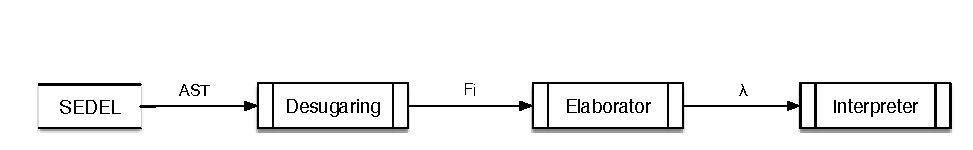
\includegraphics[scale=0.9]{pipeline.eps}
  \caption{The pipeline of \name}
  \label{fig:pipeline}
\end{figure}